\documentclass[fleqn]{minimal}

\usepackage{mathtools}
\usepackage{tikz}
\usepackage{color}

\usetikzlibrary{shapes, backgrounds}

\begin{document}

\section{Setup}

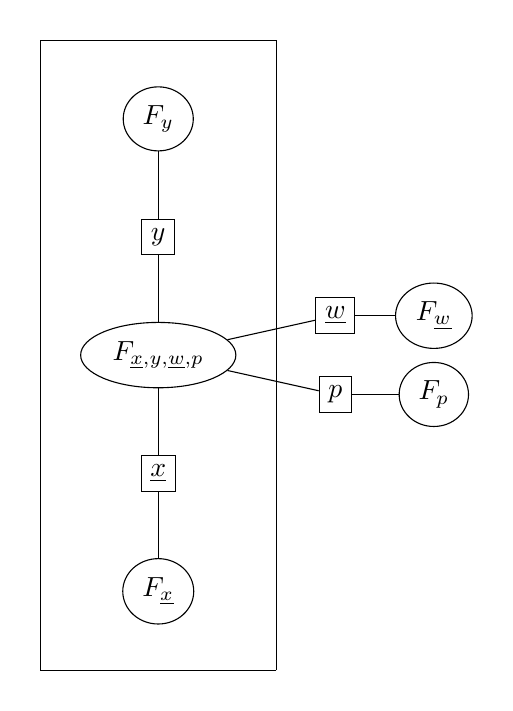
\begin{tikzpicture}
  \tikzset{background rectangle/.style={fill=white}}
  \tikzset{show background rectangle}
  
  \tikzset{factor/.style={ellipse, draw}}
  \tikzset{sepset/.style={rectangle, draw}}
  
  \node[factor] (Fx) at (0.0,0.0) {$F_{\underline{x}}$};
  \node[sepset] (x) at (0.0,1.5) {$\underline{x}$};
  \node[factor] (Fxywp) at (0.0,3.0) {$F_{\underline{x}, y, \underline{w}, p}$};
  \node[sepset] (y) at (0.0,4.5) {$y$};
  \node[factor] (Fy) at (0.0,6.0) {$F_{y}$};

  \draw (-1.5,-1.0) -- (-1.5, 7.0);
  \draw (-1.5, 7.0) -- ( 1.5, 7.0);
  \draw ( 1.5, 7.0) -- ( 1.5,-1.0);
  \draw ( 1.5,-1.0) -- (-1.5,-1.0);

  \node[sepset] (w) at (2.25,3.5) {$\underline{w}$};
  \node[factor] (Fw) at (3.5,3.5) {$F_{\underline{w}}$};
  \node[sepset] (p) at (2.25,2.5) {$p$};
  \node[factor] (Fp) at (3.5,2.5) {$F_{p}$};

  \draw (Fx) -- (x);
  \draw (x) -- (Fxywp);
  \draw (Fxywp) -- (y);
  \draw (y) -- (Fy);
  \draw (Fxywp) -- (p);
  \draw (Fxywp) -- (w);
  \draw (p) -- (Fp);
  \draw (w) -- (Fw);
\end{tikzpicture}

\textbf{With}

\begin{align*}
  F_{\underline{x}}
  & = N_{\underline{x}}
  \left(
    \underline{\mu} ;
    \Sigma
  \right) \\
  & = \dfrac{1}{\sqrt{2\pi}}
  \left| \Sigma \right|^{-1/2}
  \exp
  \left\{
    - \dfrac{1}{2}
    \left( \underline{x} - \underline{\mu}\right)'
    \Sigma^{-1}
    \left( \underline{x} - \underline{\mu}\right)
  \right\}
\end{align*}

\begin{align*}
  F_{y}
  & = N_{y}
  \left(
    \tau ;
    \lambda
  \right) \\
  & = \dfrac{1}{\sqrt{2\pi\lambda}}
  \exp
  \left\{
    - \dfrac{1}{2\lambda}
    \left(y - \tau\right)^2
  \right\}
\end{align*}

\begin{align*}
  F_{\underline{w}}
  & = N_{\underline{w}}
  \left(
    \underline{\theta} ;
    \Phi
  \right) \\
  & = \dfrac{1}{\sqrt{2\pi}}
  \left| \Phi \right|^{-1/2}
  \exp
  \left\{
    - \dfrac{1}{2}
    \left( \underline{w} - \underline{\theta}\right)'
    \Phi^{-1}
    \left( \underline{w} - \underline{\theta}\right)
  \right\}
\end{align*}

\begin{align*}
  F_{p}
  & = \Gamma_p
  \left(
    \nu ;
    \psi
  \right) \\
  & = \dfrac{1}{\psi^\nu \Gamma(\nu)}
  p^{\nu-1}
  exp
  \left\{
    - \dfrac{p}{\psi}
  \right\}
\end{align*}

\begin{align*}
  F_{\underline{x}, y, \underline{w}, p}
  & = N_y
  \left(
    \underline{x}'\underline{w} ;
    p^{-1}
  \right) \\
  & =\dfrac{\sqrt{p}}{\sqrt{2\pi}}
  exp
  \left\{
    - \dfrac{p}{2}
    \left( y - \underline{x}'\underline{w} \right)^2
  \right\}
\end{align*}

\subsection{Calculate belief on $F_{\underline{x}, y, \underline{w}, p}$}

\begin{align*}
  B\left(F_{\underline{x}, y, \underline{w}, p}\right)
  & = \dfrac{\sqrt{p}}{\sqrt{2\pi}}
  exp
  \left\{
    - \dfrac{p}{2}
    \left( y - \underline{x}'\underline{w} \right)^2
  \right\} \\
  & \times
  M\left(F_{\underline{x}} \rightarrow F_{\underline{x}, y, \underline{w}, p}\right)
  M\left(F_{y} \rightarrow F_{\underline{x}, y, \underline{w}, p}\right)
  M\left(F_{\underline{w}} \rightarrow F_{\underline{x}, y, \underline{w}, p}\right)
  M\left(F_{p} \rightarrow F_{\underline{x}, y, \underline{w}, p}\right)
\end{align*}

\begin{align*}
  B\left(F_{\underline{x}, y, \underline{w}, p}\right)
  & = \dfrac{\sqrt{p}}{\sqrt{2\pi}}
  exp
  \left\{
    - \dfrac{p}{2}
    \left( y - \underline{x}'\underline{w} \right)^2
  \right\} \\
  & \times
  \dfrac{1}{\sqrt{2\pi}}
  \left| \Sigma \right|^{-1/2}
  \exp
  \left\{
    - \dfrac{1}{2}
    \left( \underline{x} - \underline{\mu}\right)'
    \Sigma^{-1}
    \left( \underline{x} - \underline{\mu}\right)
  \right\} \\
  & \times
  \dfrac{1}{\sqrt{2\pi\lambda}}
  \exp
  \left\{
    - \dfrac{1}{2\lambda}
    \left(y - \tau\right)^2
  \right\} \\
  & \times
  \dfrac{1}{\sqrt{2\pi}}
  \left| \Phi \right|^{-1/2}
  \exp
  \left\{
    - \dfrac{1}{2}
    \left( \underline{w} - \underline{\theta}\right)'
    \Phi^{-1}
    \left( \underline{w} - \underline{\theta}\right)
  \right\} \\
  & \times
  \dfrac{1}{\psi^\nu \Gamma(\nu)}
  p^{\nu-1}
  exp
  \left\{
    - \dfrac{p}{\psi}
  \right\}
\end{align*}

\end{document}
